\documentclass{beamer}
\usepackage{amsmath}
\usepackage{enumerate}
\usepackage[makeroom]{cancel} % ������������
\usepackage{multicol,multirow} %��������� �������
\usepackage{hyperref}
\usepackage{tabularx}
\usepackage{amsfonts}
\usepackage{amssymb}
\usepackage{amsmath}
\DeclareMathOperator{\Tr}{Tr}
\DeclareMathOperator{\diag}{diag}
\DeclareMathOperator{\conv}{conv}
\DeclareMathOperator{\Rg}{Rg}
\DeclareMathOperator{\Ker}{Ker}
\newcommand{\matrixl}{\left|\left|}
\newcommand{\cbad}{c_{\mathrm{bad}}}
\newcommand{\matrixr}{\right|\right|}
\DeclareMathOperator*{\argmin}{arg\,min}
\DeclareMathOperator*{\supp}{supp}
\newcommand{\h}{\mathbf{h}}
\newcommand{\x}{\mathbf{x}}
\newcommand{\aaa}{\mathbf{a}}
\newcommand{\w}{\mathbf{w}}
\newcommand{\W}{\mathbf{W}}
\newcommand{\y}{\mathbf{y}}
\newcommand{\X}{\mathbf{X}}
\newcommand{\Y}{\mathbf{Y}}
\newcommand{\fx}{\mathbf{f}}
\newcommand{\fs}{\mbox{f}}
\usepackage[cp1251]{inputenc}
\usepackage[russian]{babel}
\usepackage{amsmath,mathrsfs,mathtext}
\usepackage{graphicx, epsfig}
\usetheme{Warsaw}%{Singapore}%{Warsaw}%{Warsaw}%{Darmstadt}
\usecolortheme{sidebartab}
\definecolor{beamer@blendedblue}{RGB}{55,172,32}
%----------------------------------------------------------------------------------------------------------
\title[\hbox to 56mm{Classifying distributions \hfill\insertframenumber\,/\,\inserttotalframenumber}]
{Classifying probabilistic distributions}
\author[S.E. Volodin]{\large \\S.E. Volodin}
\institute{\large MIPT}

\date{}
%-------------------------------------------------------
\begin{document}
%-------------------------------------------------------
\begin{frame}
%\thispagestyle{empty}
\titlepage
\end{frame}
%-------------------------------------------------------
\begin{frame}{The dataset}
\begin{enumerate}
\item Probability distributions $\{f_k(x)\colon\mathbb{R}\to\mathbb{R}\}_{k=1}^K$
\item Picking one of them $k\in\overline{1,K}$
\item Picking points $[a,b]\subseteq \mbox{Dom} f_k$
\item Dividing $[a,b]$ into 101 parts: $[a,b]=\bigsqcup\limits_{s=0}^{100}\Delta_s$, $$|\Delta_0|=|\Delta_{100}|=\frac{\Delta_s}{2}$$
\item Sampling $t_z\sim f_k$
\item Counting numbers in $\Delta_s$: $x^i_s=\sum\limits_z[t_z\in\Delta_s]$

\end{enumerate}
\centering $\Rightarrow$ Obtained object $\{x_s\}\in\mathfrak{D}$
\end{frame}
\begin{frame}{The dataset}
Answers: $y_i=[k=\hat{k}]$ for a fixed $\hat{k}$.
$$f_{\hat{k}}=ax^{a-1}\big[x\in[0,1]\big]$$
\begin{tabular}{cc}
\begin{minipage}{0.5\textwidth}\begin{figure}
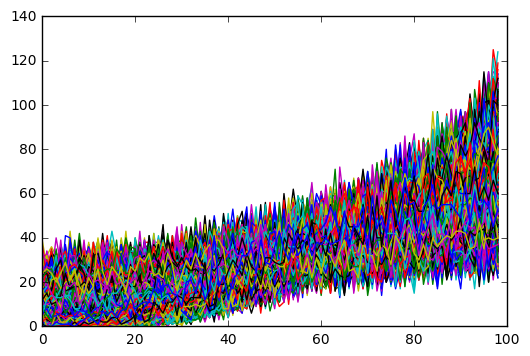
\includegraphics[width=150px]{0.png} 
\caption{1. Training set, $y_i=0$}
\end{figure}\end{minipage} &
\begin{minipage}{0.5\textwidth}\begin{figure}
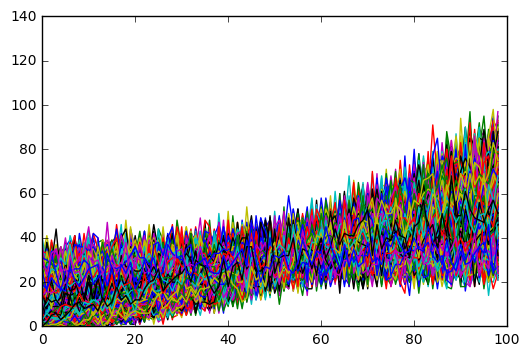
\includegraphics[width=150px]{1.png}
\caption{2. Training set, $y_i=1$}
\end{figure}\end{minipage}
\end{tabular}
\end{frame}
\begin{frame}{The solution}
Idea: dimension reduction
\begin{enumerate}
\item Fitting a polynom
$\sum |P_n(s)-x_s|^2\to\min$
{\centering 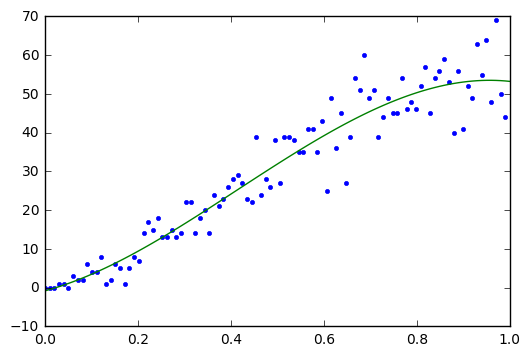
\includegraphics[width=200px]{fit}}
\item Using coefficients $\mbox{coeff}(P_n)$ as features of $\{x^i_s\}\in\mathfrak{D}$
\end{enumerate}
\end{frame}
\begin{frame}{Choosing degree}
5-fold cross-validation
	\centering 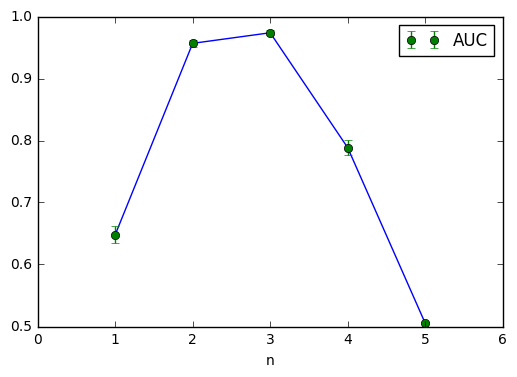
\includegraphics[width=250px]{AUC_n}
\\
{\bf Answer:} $n^*=3$
\end{frame}
\begin{frame}{Result}
\centering 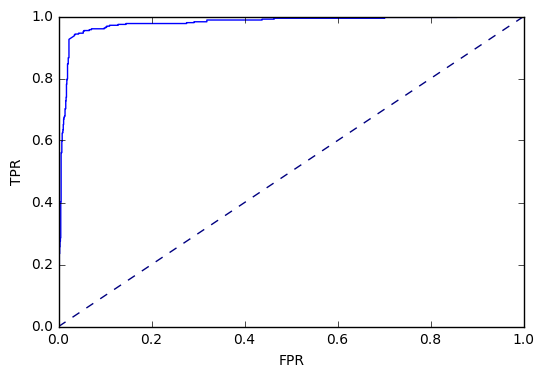
\includegraphics[width=250px]{auc}
\end{frame}
\begin{frame}{Result}
\centering 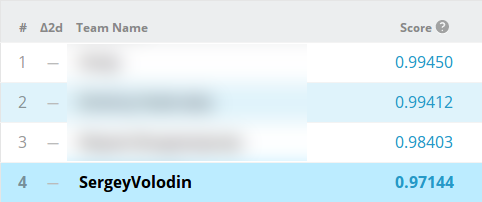
\includegraphics[width=250px]{res}
\end{frame}
\begin{frame}{The end}
\centering
\Huge{Thank you!\\Questions?}
\end{frame}
\end{document}